\documentclass[a4paper,12pt]{book} % nie: report!


% pakiety
\usepackage{polski} % lepiej to zamiast babel!
\usepackage[utf8]{inputenc} % w razie kłopotów spróbować: \usepackage[utf8x]{inputenc}
\usepackage{fancyhdr} % nagłówki i stopki
\usepackage{indentfirst} % WAŻNE, MA BYĆ!
\usepackage{lipsum}
\usepackage[pdftex]{graphicx} % to do wstawiania rysunków
\usepackage{amsmath} % to do dodatkowych symboli, przydatne
\usepackage[pdftex,
            left=1in,right=1in,
            top=1in,bottom=1in]{geometry} % marginsy
\usepackage{amssymb} % to też do dodatkowych symboli, też przydatne
\usepackage{pdfpages} % żeby wstawić stronę tytułową
% jesli potrzeb, można oczywiście wstawić inne pakiety i swoje definicje...
  

% definicje nagłówków i stopek
\pagestyle{fancy}
\renewcommand{\chaptermark}[1]{\markboth{#1}{}}
\renewcommand{\sectionmark}[1]{\markright{\thesection\ #1}}
\fancyhf{}
\fancyhead[LE,RO]{\footnotesize\bfseries\thepage}
\fancyhead[LO]{\footnotesize\rightmark}
\fancyhead[RE]{\footnotesize\leftmark}
\renewcommand{\headrulewidth}{0.5pt}
\renewcommand{\footrulewidth}{0pt}
\addtolength{\headheight}{1.5pt}
\fancypagestyle{plain}{\fancyhead{}\cfoot{\footnotesize\bfseries\thepage}\renewcommand{\headrulewidth}{0pt}}

% interlinia
\linespread{1.25}


% treść
\begin{document}
\sloppy



\thispagestyle{empty}

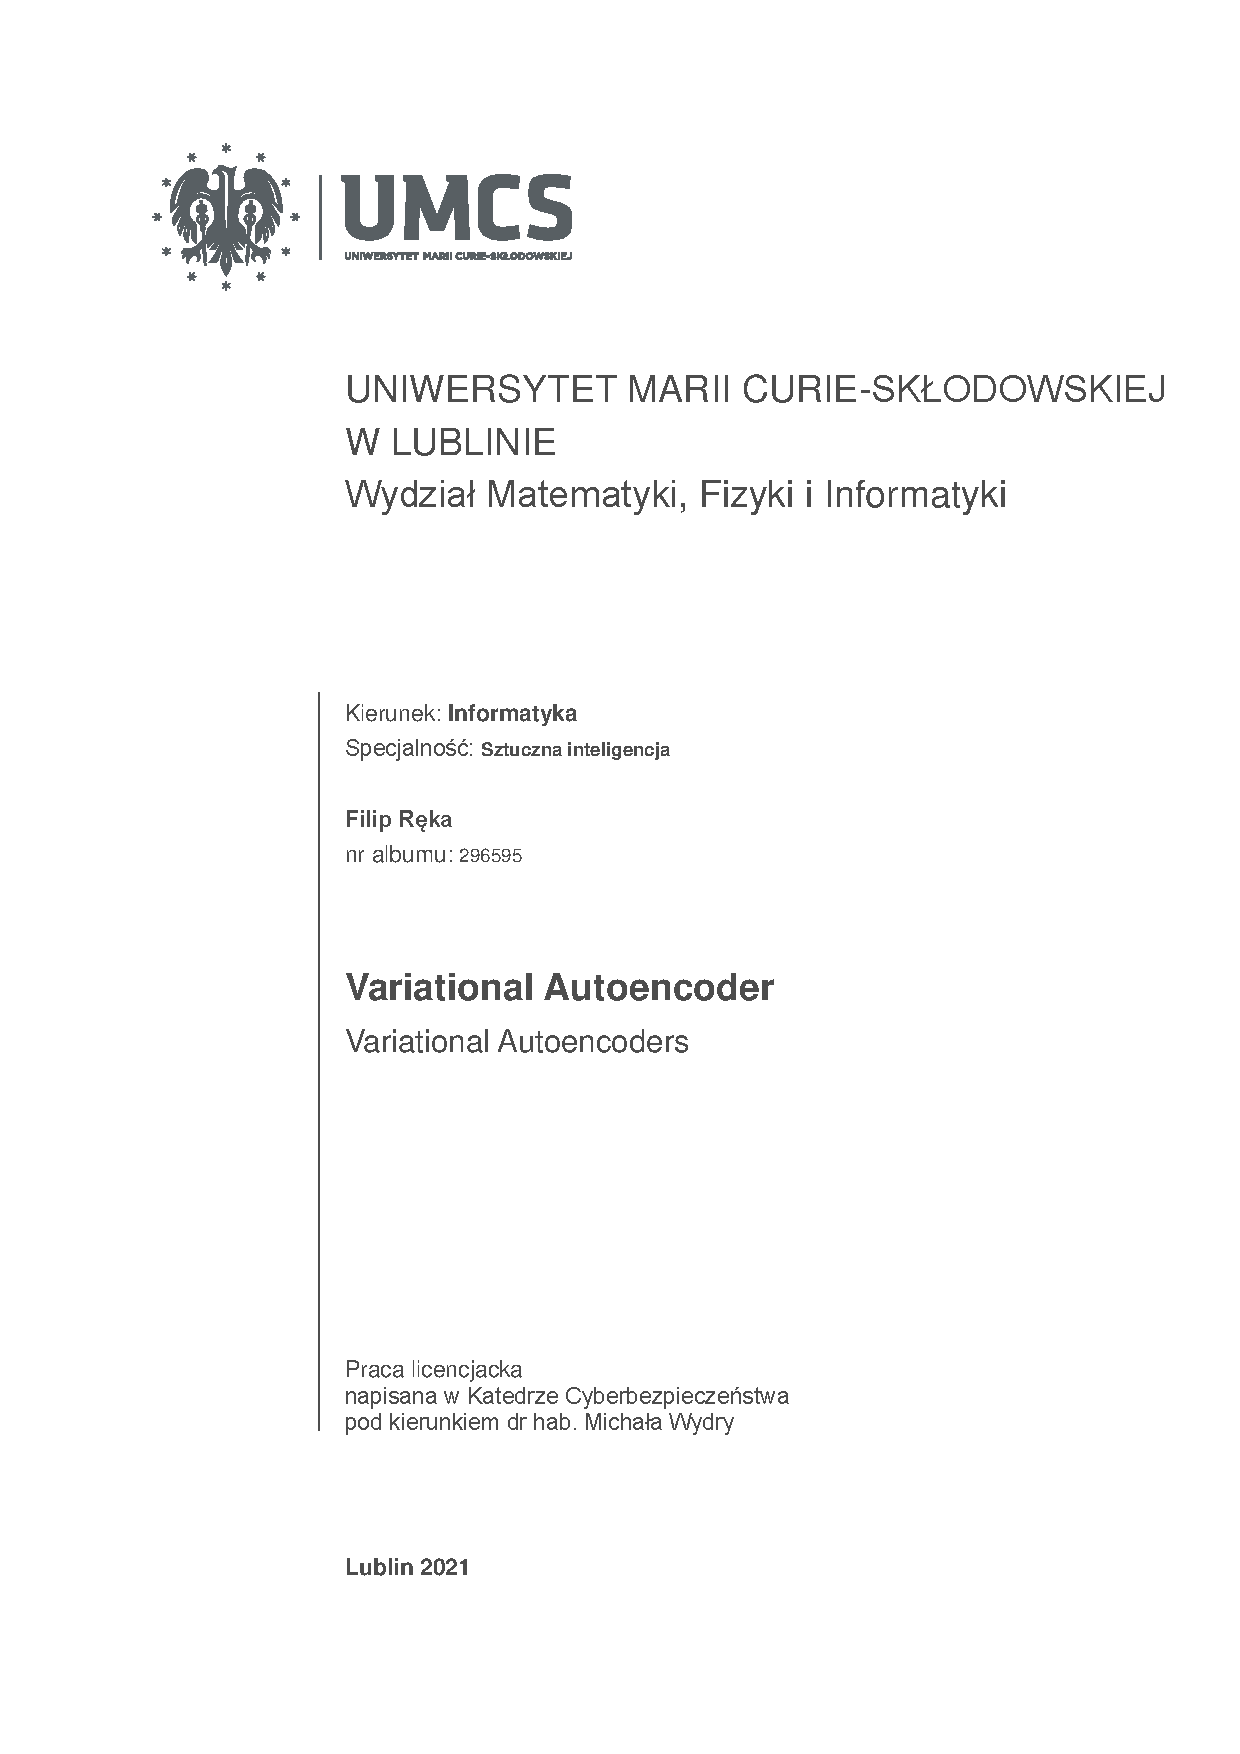
\includepdf{stronatytulowasvg}
% najpierw uzupełnij w 'stronatytulowa.odt' openoffice i wyeksportuj do 'stronatytulowa.pdf'


\thispagestyle{empty}

\tableofcontents{}

\chapter*{Wstęp} % z gwiazdką, więc bez numerka...
\addcontentsline{toc}{chapter}{Wstęp} % ...ale w spisie treści ma być
\textbf{Wariacyjne Autoenkodery} stają się coraz bardziej popularnymi modelami uczenia maszynowego. Zostały zaproponowane przez Diederika P Kingma i Maxa Wellinga. Najczęściej zostają one skategoryzowane do modeli uczenia częściowo nadzorowanego. Znajdują zastosowanie w generacji obrazów, tekstu, muzyki, odszumianiu obrazków, sygnałów oraz w detekcji anomalii. W przeciwieństwie do tradycyjnych autoenkoderów prezentują pobabilistyczne podejście do generowania zmiennych ukrytych. Swoją popularność zawdzięcza swojej budowie, która jest oparta na sieciach neuronowych oraz możliwości trenowania go przy pomocy metod gradientowych.
\chapter{Tradycyjny a wariacyjny autoenkoder} 
\section{Autoencoder}
\subsection{Informacje ogólne}
Autoencoder składa się z dwóch części: enkodera , który koduje dane wejściowe oraz dekodera, który na podstawie kodu rekonstruuje wejście. Architektura enkodera wymaga aby jego warstwa wyjściowa generująca reprezentacje danych była mniejsza niż warstwa wejściowa. W innym przypadku sieć po prostu przekopiowałaby wejście. Często to zwężenie nazywa się mianem \textit{bottle neck}. Celem treningu całego autoenkodera jest zminimalizowanie błędu pomiędzy wejściem a wyjściem. W przypadku obrazów funkcją straty może być na przykład błąd średniokwadratowy. \\
Powiedzmy że mamy dane wejściowe $X$ o wymiarze $m$ oraz chcemy je zakodować do wymiaru $n$. Formalnie możemy zapisać, że model próbuje nauczyć się funkcji: \\ 
\begin{center}
	Enkoder $A : \mathbb{R}^m \rightarrow \mathbb{R}^n$\\
	Dekoder $B: \mathbb{R}^n \rightarrow \mathbb{R}^m$
\end{center}
Funkcją straty naszego modelu, którą będziemy chcieli zminimalizować, będzie błąd rekonstrukcji danych wejściowych i do tego celu użyjemy błędu średniokwadratowego. 
\begin{center}
	$\mathcal{L}(x, x') = \dfrac{1}{m}\displaystyle\sum_{i=0}^{m}(x_i-x'_i)^2 = \dfrac{1}{m}\displaystyle\sum_{i=0}^{m}(x_i-B(A(x_i)))^2$
\end{center}
\subsection{Zastosowanie}
Dwoma głównymi zastosowaniami tradycyjnych autoenkoderów są:
\begin{itemize}
	\item Odszumianie
	\item Redukcja wymiarów 
\end{itemize}
\subsection{Problemy z generacją nowych danych}
Dobrym pytaniem jest czy przy pomocy kodu jesteśmy generować nowe dane bardzo podobne do tych co model otrzymał na wejściu. Aby model mógł generować nowe dane muszą zostać spełnione dwa warunki:
\begin{itemize}
	\item Nasza przestrzeń kodu (tzw. zmiennych ukrytych) musi być ciągła co znaczy że dwa punkty znajdujące się obok siebie będą dawać podobne dane jak zostaną odkodowane
	\item Przestrzeń musi być kompletna co znaczy, ze punkty wzięte z dystrybucji muszą dawaj wyniki mające sens
\end{itemize}
Korzystając z tradycyjnych autoenkoderów nie mamy zagwarantowanego, że oba te kryteria zostaną spełnione.\\

Zwykłe autoenkodery po prostu nie nadają się do generacji danych ponieważ nigdy nie zostały do tego stworzone. Ich głównym celem jest jak najlepsze odzwierciedlenie danych ze zmiennych ukrytych. 
\section{Wariacyjny autoenkoder}
\subsection{Różnice}
Wariacyjny autoenkoder ma inne podejście do generowania zmiennych ukrytych. Zamiast generować jedną zmienną dla każdego wymiaru, generuje dwie liczby, $\sigma$ oraz $\mu$, które traktujemy jako odchylenie standardowe oraz średnią rozkładu normalnego.
Dla przykładu jeśli uznamy ze chcemy dane reprezentować jako siedmio-wymiarowy wektor, nasz enkoder wygeneruje dwa wektory siedmio-wymiarowe, z którego jeden będzie przechowywał wartości średniej a drugi odchylenia standardowego dla każdego z siedmiu rozkładu normalnego. Kolejną istotną zmiana jest funkcja straty, która oprócz błędu rekonstrukcji obrazu składa się z dywergencji Kullbacka-Leiblera.\\
\chapter{Wariacyjny autoenkoder}
\section{Teoria za modelem VAE}
\subsection{Motywacja statystyczna}
Powiedzmy ze istnieje zmienna ukryta $z$, która generuje obserwację $x$. Mamy tylko informację o $x$ i chcemy się dowiedzieć jakiej jest $z$. Aby to zrobić powinniśmy policzyć $p(z|x)$. Z twierdzenia Bayesa wiemy że:\\
\begin{center}
	$p(z|x)=\dfrac{p(x|z)p(z)}{p(x)}$
\end{center}
Aby obliczyć rozkład marginalny $p(x)$ musimy policzyć:
\begin{center}
	$p(x) = \displaystyle\int_{z}^{}p(x,z)dz$
\end{center}
Obliczenie tej całki jest bardzo trudne ponieważ $z$ jest często wielowymiarowe i przestrzeń przeszukiwań jest zwyczajnie kombinatorycznie za duża aby korzystać z takich metod jak próbkowanie Monte Carlo łańcuchami Markowa. \\

\section{Wnioskowanie wariacyjne}
Rozwiązaniem tego problemu jest próba policzenia rozkładu $q(z|x)$, które będzie jak najlepiej odzwierciedlać $p(z|x)$ i będzie miał rozkład, który będziemy mogli policzyć. 
\subsection{Dywergencji Kullbacka-Leiblera}
Jest to miara określająca rozbieżność między dwoma rozkładami prawdopodobieństwa. Nie można określić jej mianem metryki ponieważ nie jest symetryczna ($D_{KL}(P\|Q)\neq  D_{KL}(Q\|P)$).\\ Naszym celem będzie zminimalizowanie jej.
\begin{center}
	$q^\ast(z|x)=\operatorname*{argmin}_{q(z|x)\in Q}(D_{KL}(q(z|x)\|p(z|x)))$
	\\gdzie $Q$ to rodzina prostych dystrybucji, na przykład rozkładu Gaussa 
\end{center}
Policzmy:
\begin{center}
	$D_{KL}(q(z|x)\|p(z|x))=\mathbb{E}_{z\sim q(z|x)}\log\dfrac{p(z|x)}{q(z|x)} = 
	\displaystyle\int_{z}^{}q(z|x)\log\frac{q(z|x)}{p(z|x)}dz$
\end{center}
	 Natrafiamy na kolejny problem ponieważ nie możemy $p(z|x)$ jednak jesteśmy w stanie to przepisać jako:\\
\begin{center}
	$p(z|x)=\dfrac{p(z,x)}{p(x)}$
\end{center}
Tu jest dużo matmy której nie chce mi się na razie pisać ale tu będzie ELBO.
\newpage
W naszym przypadku będziemy chcieli aby $q$ było rozkładem normalnym co znaczy że
\chapter{Kolejny rozdział o niczym}
\section{Pozdrowienia do więzienia}
\lipsum[1]\cite{doersch2021tutorial}

\listoftables{} % jeśli są tabele
\addcontentsline{toc}{chapter}{Spis tabel}

\listoffigures{} % jeśli są tabele
\addcontentsline{toc}{chapter}{Spis rysunków}

\bibliographystyle{ieeetr}
\bibliography{./cytowania/cytowania.bib}


%\begin{thebibliography}{99}
%\addcontentsline{toc}{chapter}{Bibliografia}
% \bibitem aaaaaaaa
% \bibitem bbbbbbbb 
%\end{thebibliography}


\end{document}
